\documentclass[../../Orator]{subfiles}
\begin{document} 
 
% Make a table of symbols
% We need to figure out how much biology analogues should be in here

\section{Circuits}
The circuit for the Hodgkin-Huxley model can be seen in \Cref{fig:HH circuit}. 

\begin{figure}[h]
    \centering
    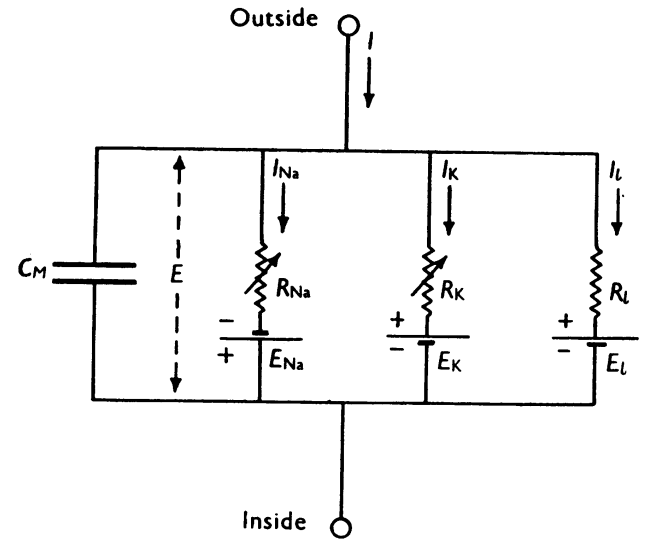
\includegraphics[width=300 pt]{Pictures/Alex/Hodgkin-Huxley model 2.png}
    \caption{The circuit diagram of the Hodgkin-Huxley model \cite{}.}
    \label{fig:HH circuit}
\end{figure}

There are five elements to this circuit diagram. These are the batteries, capacitor, resistor, variable resistors, and wires. 

The batteries are symbolised by two parallel lines where one is longer than the other. The shorter end is the negative side (anode) and the longer end is the positive side (cathode). In this model, there are three batteries placed in different directions. The task of the batteries is to store energy and push said energy through the wires. When batteries are placed in parallel like this, the voltage does not get increased. However, the current capacity increases, so the batteries last longer. The unit of batteries is watt-hours (Wh) or milliamp-hours (mAh) \cite{}. 

The symbol for the capacitor is two parallel lines of equal length. Much like the batteries, the capacitor stores electrical charge. However, a capacitor cannot store as much energy as a comparable-sized battery. But in return, capacitors can charge and discharge faster. Capacitance is measured in Farads (\unit{\farad}) \cite{}.

Resistors are represented by zig-zag lines. These work against the batteries and the resistor as it removes energy from the equation and turns it into heat. The resistor has a fixed value of resistance. This is measured in ohms (\unit{\ohm}) \cite{}.

Variable resistors, also called varistors, are a type of resistor. These are also represented by a zig-zag line, however, they have an arrow through them. Unlike the normal resistor, the varistors have almost infinite resistance before a certain voltage. Here they act like an insulator allowing almost no current through. After it has reached a certain voltage, it slowly starts to act like a conductor, having almost no resistance \cite{}. 

The lines connecting the pieces together are the wires. Much like what is shown in the figure, the wires connect all the parts of the model. The wires are in theory considered to have no resistance. But in reality, they always have some, even if it is very little \cite{}. 


 \section{Voltage + Current}
%\(v = iR\)
The flow of charge is called current. Current is measured by the number of charges that pass through a boundary per unit of time. The symbol for current is I and its unit is Ampere. The formula for current is derived from Ohm's law. Ohm's law is \(V=IR\), where \(V\) is the voltage, \(I\) is the current, and \(R\) is the resistance. Voltage is synonymous with electric pressure. This pressure pushes the current through a loop in order for it to produce some kind of work \cite{}. 


\section{Ions, disambigious}

%\begin{theorem}
%    \label{th:complex analysis}
%    2+2 = x, 3 < x < 5
%\end{theorem}

%\begin{equation}
%55 - 3 \leq 100
%\label{eq:math}
%\end{equation}



\end{document}